\documentclass{beamer}
\usetheme{Warsaw}

\usepackage[utf8]{inputenc}
\usepackage{fancybox}
\usepackage{multimedia} 
\usepackage{subfig}
\usepackage{amsmath}
\usepackage{hyperref}
\usepackage[all]{xy}
\usepackage{algorithm}
%\usepackage{arevmath}     % For math symbols
\usepackage[noend]{algpseudocode}

\begin{document}


\title[Angewandte Mathematik] % (optional, only for long titles)
{Angewandte Mathematik
\\
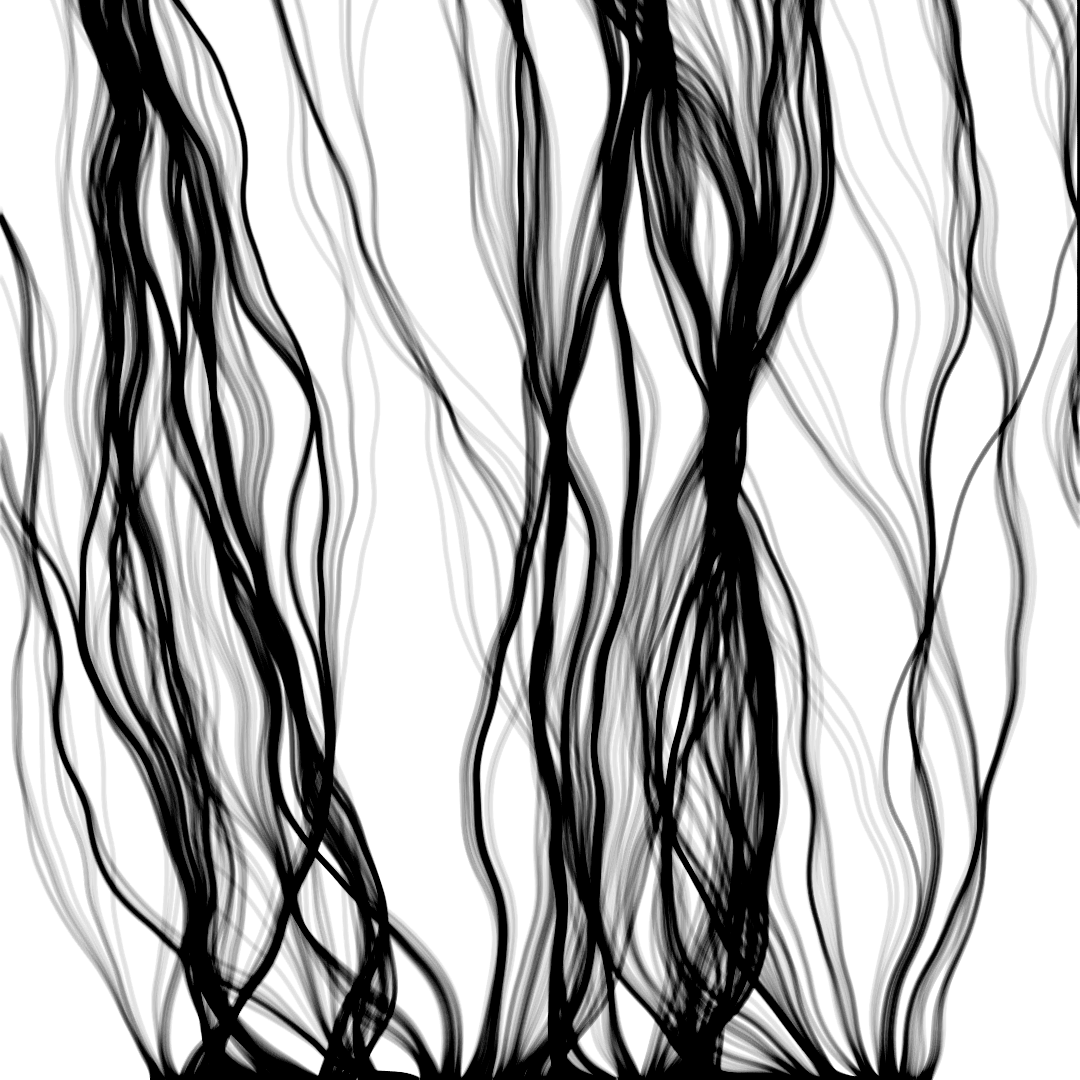
\includegraphics[scale=0.15]{images/cover}
}
\subtitle{}
\author[Dr. Johannes Riesterer] % (optional, for multiple authors)
{Dr.  rer. nat. Johannes Riesterer}

\date[KPT 2004] % (optional)
{}

\subject{Angewandte Mathematik}



\frame{\titlepage}



\begin{frame}
    \frametitle{Angewandte Mathematik}
\framesubtitle{Dynamische Systeme }
\begin{block}{Gedämpftes Pendel}
$\theta''(t) = -L \theta - \underbrace{\mu \theta'}_{\text{drag}}$. $L \theta = mg \sin(\theta)$ 
\end{block}
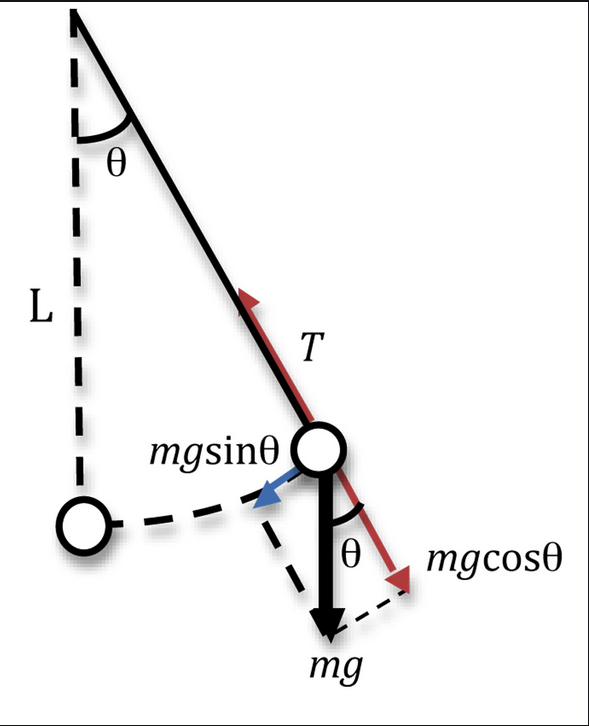
\includegraphics[scale=0.2]{images/pendulum0}
\begin{block}{System gedämpftes Pendel}
    $ \frac{d}{dt}\begin{pmatrix}
        x_1(t) \\ x_2(t)
    \end{pmatrix} = 
    \begin{pmatrix}
        x_2(t) \\ -\mu x_1(t) - \frac{m g}{L} \sin(x_2(t))  
    \end{pmatrix} $ (nicht linear!)
    \end{block}
 \end{frame}

 \begin{frame}
    \begin{block}{Phasenbild gedämpftes Pendel}
    $\mu = 0$
    \frametitle{Angewandte Mathematik}
\framesubtitle{Dynamische Systeme }
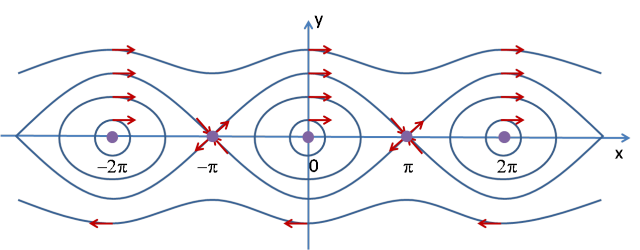
\includegraphics[scale=0.9]{images/pendulum1}
    \end{block}
\end{frame}

\begin{frame}
    \frametitle{Angewandte Mathematik}
\framesubtitle{Dynamische Systeme }
\begin{block}{Harmonischer Oszillator}
\begin{align*}
    \frac{d}{dt}\begin{pmatrix}
        x_1(t) \\ x_2(t)
    \end{pmatrix} = 
\begin{pmatrix}
    0 & -1  \\ 1 & 0
\end{pmatrix} \cdot
\begin{pmatrix} 
    x_1(t) \\ x_2(t)
\end{pmatrix} 
\end{align*}
\end{block}

\begin{block}{Lösung Harmonischer Oszillator}
    Anfangswert $\begin{pmatrix}
        x_1 \\ x_2\end{pmatrix} = \begin{pmatrix}
            x_1(t_0) \\ x_2(t_0)\end{pmatrix}$
    \begin{align*}
        \begin{pmatrix}
            x_1(t) \\ x_2(t)
        \end{pmatrix} = e^{ \begin{pmatrix}
            0 & -1  \\ 1 & 0
        \end{pmatrix} t } \cdot \begin{pmatrix}
            x_1\\ x_2
        \end{pmatrix}
    \end{align*}
\end{block}

 \end{frame}


 \begin{frame}
    \frametitle{Angewandte Mathematik}
\framesubtitle{Dynamische Systeme }
\begin{block}{Harmonischer Oszillator}

\begin{align*}
 e^{ \begin{pmatrix}
        0 & -1  \\ 1 & 0
    \end{pmatrix} t } = \sum_{k= 0}^{n} \begin{pmatrix}
    0 & -1  \\ 1 & 0
\end{pmatrix}^{k} \frac{t^k}{k!} 
\end{align*}

\end{block}
 \end{frame}


 \begin{frame}
    \frametitle{Angewandte Mathematik}
\framesubtitle{Dynamische Systeme }
\begin{block}{Harmonischer Oszillator}

\begin{align*}
\begin{pmatrix}
        0 & -1  \\ 1 & 0
    \end{pmatrix}^{k}  = \begin{cases} 
        \begin{pmatrix}
            1 & 0  \\ 0 & 1
        \end{pmatrix}; k = 0 \mod 4 \\
        \begin{pmatrix}
            0 & -1  \\ 1 & 0
        \end{pmatrix}; k = 1 \mod 4 \\
        \begin{pmatrix}
            -1 & 0  \\ 0 & -1
        \end{pmatrix}; k = 2 \mod 4 \\
        \begin{pmatrix}
            0 & 1  \\ -1 & 0
        \end{pmatrix}; k = 3 \mod 4
    \end{cases}
\end{align*}
\end{block}
 \end{frame}

 \begin{frame}
    \frametitle{Angewandte Mathematik}
\framesubtitle{Dynamische Systeme }
\begin{block}{Harmonischer Oszillator}

\begin{align*}
\sum_{k= 0}^{n} \begin{pmatrix}
    0 & -1  \\ 1 & 0
\end{pmatrix}^{k} \frac{t^k}{k!} & =
\begin{pmatrix}
    1-\frac{t^2}{2!} + \frac{t^4}{4!}-\frac{t^6}{6!} \cdots & -t +\frac{t^3}{3!} - \frac{t^5}{5!} +\frac{t^7}{7!} \cdots  \\ 1 & 0 \\
    t -\frac{t^3}{3!} + \frac{t^5}{5!} -\frac{t^7}{7!} \cdots  & 1-\frac{t^2}{2!} + \frac{t^4}{4!}-\frac{t^6}{6!}  \cdots
\end{pmatrix} \\
&= \begin{pmatrix}
    \cos(t) & -\sin(t)  \\ \sin(t) & \cos(t)
\end{pmatrix}
\end{align*}
\href{https://de.wikipedia.org/wiki/Taylorreihe}{Link:Trigonometrische Taylorreihen}
\end{block}
 \end{frame}




 \begin{frame}
    \frametitle{Angewandte Mathematik}
\framesubtitle{Dynamische Systeme }

\begin{block}{Lösung Harmonischer Oszillator}
  
    \begin{align*}
        \begin{pmatrix}
            x_1(t) \\ x_2(t)
        \end{pmatrix} = \begin{pmatrix}
            \cos(t) & -\sin(t)  \\ \sin(t) & \cos(t)
        \end{pmatrix}   \cdot \begin{pmatrix}
            x_1\\ x_2
        \end{pmatrix}
    \end{align*}
\end{block}
\center
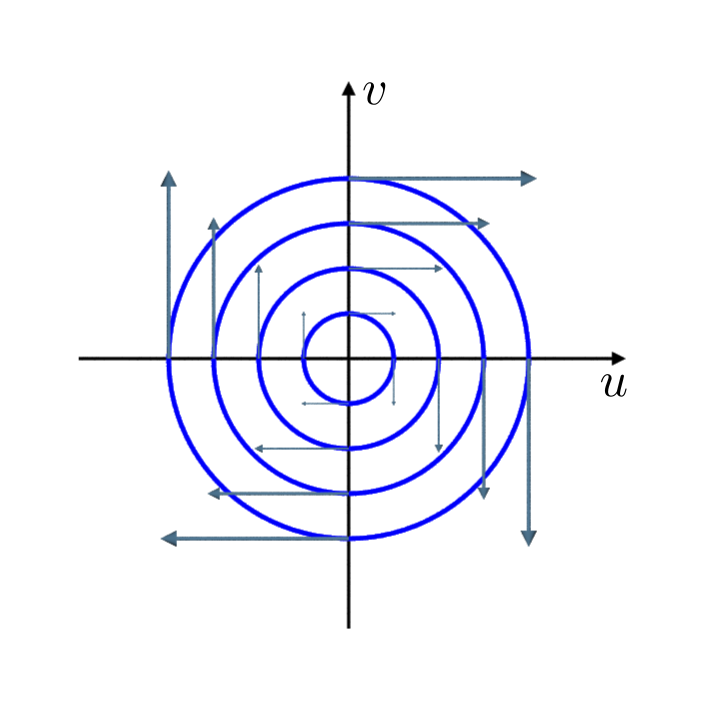
\includegraphics[scale=0.25]{images/harmonicoszillatorphasespace}
 \end{frame}



 \begin{frame}
    \frametitle{Angewandte Mathematik}
\framesubtitle{Dynamische Systeme }

\begin{block}{Harmonischer Oszillator Eigenwerte}
    \begin{align*}
    \det (\begin{pmatrix}
        0 & -1  \\ 1 & 0
    \end{pmatrix} - \lambda E) = 
    \det \begin{pmatrix}
        -\lambda & -1  \\ 1 & -\lambda  
    \end{pmatrix} = \lambda^2 +1 \Rightarrow \lambda_{1,2} = \pm i
\end{align*}
Komplexer Eigenwert.
 \end{block}
 \end{frame}


 \begin{frame}
    \frametitle{Angewandte Mathematik}
\framesubtitle{Dynamische Systeme }
\begin{block}{Lineares System mit Hauptraum}
\begin{align*}
    \frac{d}{dt}\begin{pmatrix}
        x_1(t) \\ x_2(t)
    \end{pmatrix} = 
\begin{pmatrix}
    1 & 1  \\ 1 & 0
\end{pmatrix} \cdot
\begin{pmatrix} 
    x_1(t) \\ x_2(t)
\end{pmatrix} 
\end{align*}
\end{block}

\begin{block}{Lineares System mit Hauptraum}
    \begin{align*}
    \det (\begin{pmatrix}
        1 & 1  \\ 1 & 0
    \end{pmatrix} - \lambda E) = 
    \det \begin{pmatrix}
        1-\lambda & 1  \\ 0 & 1-\lambda  
    \end{pmatrix} = (1-\lambda)^2 \Rightarrow \lambda_{1,2} = 1
\end{align*}
Doppelter Eigenwert.
\end{block}

\end{frame}

 \begin{frame}
    \frametitle{Angewandte Mathematik}
\framesubtitle{Dynamische Systeme }
\begin{block}{Eigenraum zum Eigenwert $1$}
    \begin{align*}
    \ker (\begin{pmatrix}
        1 & 1  \\ 0 & 1
    \end{pmatrix} - E) = 
    \ker \begin{pmatrix}
        0 & 1  \\ 0 & 0  
    \end{pmatrix} = \{e_1\}
\end{align*}
Doppelter Eigenwert aber Eigenraum ist eindimensional. 
 \end{block}
 \begin{block}{Hauptraum zum Eigenwert $1$}
    \begin{align*}
    \ker ( (\begin{pmatrix}
        1 & 1  \\ 0 & 1
    \end{pmatrix} - E)^2) = 
    \ker \begin{pmatrix}
        0 & 1  \\ 0 & 0  
    \end{pmatrix}^2 = \ker \begin{pmatrix}
        0 & 0  \\ 0 & 0  
    \end{pmatrix} =  \{e_1, e_2\}
\end{align*}
$e_2$ ist Hauptvektor der Stufe $2$, $e_1$ Hauptvekrot der Stufe $1$, also

$ \biggl (\begin{pmatrix}
    1 & 1  \\ 0 & 1
\end{pmatrix} - E \biggr) e_2 = e_1; \;  \biggl (\begin{pmatrix}
    1 & 1  \\ 0 & 1
\end{pmatrix} - E \biggr) e_1 = 0$ 
 \end{block}
 \end{frame}


 \begin{frame}
    \frametitle{Angewandte Mathematik}
\framesubtitle{Dynamische Systeme }

\begin{block}{Allgemeine Lösung}
    \begin{align*}
        & \varphi_1(t) := e^t \cdot e_1 = e^t \begin{pmatrix} 1 \\ 0\end{pmatrix} \\
        & \varphi_2(t) := e^t \biggl (E  +  \bigl (\begin{pmatrix} 1 & 1 \\ 0 & 1\end{pmatrix} - I\bigl)t \biggr )e_2 = e^t \begin{pmatrix} t  \\ 1 \end{pmatrix} \\
        & \varphi(t) = c_1 \varphi_1(t) +  c_2\varphi_2(t)
    \end{align*}
\end{block}
 \end{frame}


\end{document}
